\documentclass{standalone}

\usepackage{tikz}
\usetikzlibrary{shapes,backgrounds}

\begin{document}
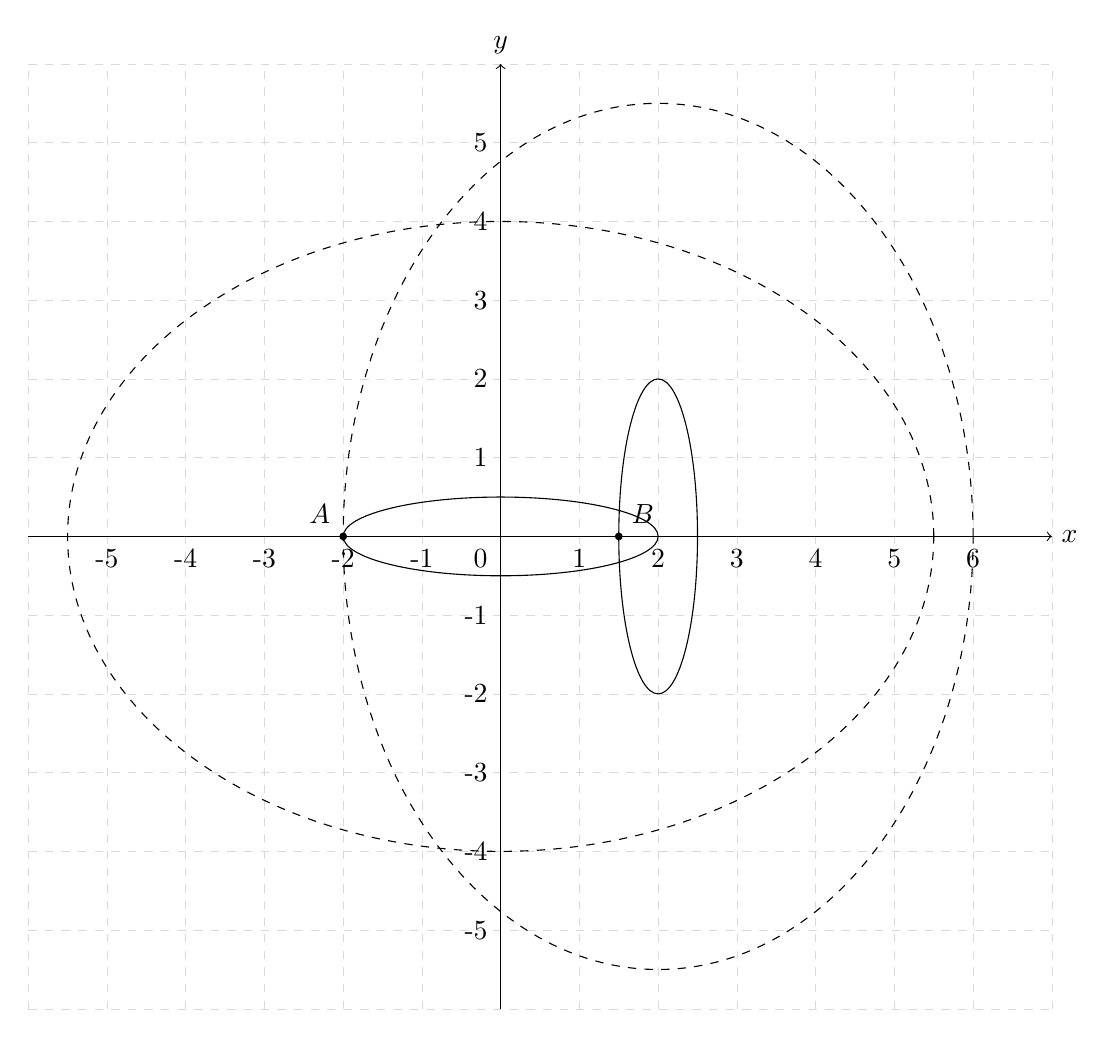
\begin{tikzpicture}
  \draw[help lines, color=gray!30, dashed] (-6,-6) grid (7,6);
  \draw[->] (-6,0)--(7,0) node[right]{$x$};
  \draw[->] (0,-6)--(0,6) node[above]{$y$};
  \node[inner sep=1pt,label=below left:{0}] at (0,0) {};
  \foreach \i in {-5,...,-1,1,2,3,4,5,6}
  {
    \node[inner sep=1pt,label=below:{\i}] at (\i,0) {};
  }
  \foreach \i in {-5,...,-1,1,2,3,4,5}
  {
    \node[inner sep=1pt,label=left:{\i}] at (0,\i) {};
  }
  \draw (0,0) ellipse (2 and 0.5);
  \draw (2,0) ellipse (0.5 and 2);
  \draw[dashed] (0,0) ellipse (5.5 and 4);
  \draw[dashed] (2,0) ellipse (4 and 5.5);
  \node[circle,inner sep=1pt,fill=black,label=above left:{$A$}] at (-2,0) {};
  \node[circle,inner sep=1pt,fill=black,label=above right:{$B$}] at (1.5,0) {};
\end{tikzpicture}
\end{document}
